\newcommand{\nom}{Porte conteneur}
\newcommand{\sequence}{03}
\newcommand{\num}{04}
\newcommand{\type}{TD}
\newcommand{\descrip}{Résolution d'un problème en utilisant des méthodes algorithmiques}
\newcommand{\competences}{Alt-C3: Concevoir un algorithme répondant à un problème précisément posé}
\documentclass[10pt,a4paper]{article}
  \usepackage[french]{babel}
  \usepackage[utf8]{inputenc}
  \usepackage[T1]{fontenc}
  \usepackage{xcolor}
  \usepackage[]{graphicx}
  \usepackage{makeidx}
  \usepackage{textcomp}
  \usepackage{amsmath}
  \usepackage{amssymb}
  \usepackage{stmaryrd}
  \usepackage{fancyhdr}
  \usepackage{lettrine}
  \usepackage{calc}
  \usepackage{boxedminipage}
  \usepackage[french,onelanguage, boxruled,linesnumbered]{algorithm2e}
  \usepackage[colorlinks=false,pdftex]{hyperref}
  \usepackage{minted}
  \usepackage{url}
  \usepackage[locale=FR]{siunitx}
  \usepackage{multicol}
  \usepackage{tikz}
  \makeindex

  %\graphicspath{{../Images/}}

%  \renewcommand\listingscaption{Programme}

  %\renewcommand{\thechapter}{\Alph{chapter}}
  \renewcommand{\thesection}{\Roman{section}}
  %\newcommand{\inter}{\vspace{0.5cm}%
  %\noindent }
  %\newcommand{\unite}{\ \textrm}
  \newcommand{\ud}{\mathrm{d}}
  \newcommand{\vect}{\overrightarrow}
  %\newcommand{\ch}{\mathrm{ch}} % cosinus hyperbolique
  %\newcommand{\sh}{\mathrm{sh}} % sinus hyperbolique

  \textwidth 160mm
  \textheight 250mm
  \hoffset=-1.70cm
  \voffset=-1.5cm
  \parindent=0cm

  \pagestyle{fancy}
  \fancyhead[L]{\bfseries {\large PTSI -- Dorian}}
  \fancyhead[C]{\bfseries{{\type} \no \numero}}
  \fancyhead[R]{\bfseries{\large Informatique}}
  \fancyfoot[C]{\thepage}
  \fancyfoot[L]{\footnotesize R. Costadoat, C. Darreye}
  \fancyfoot[R]{\small \today}
  
  \definecolor{bg}{rgb}{0.9,0.9,0.9}
  
  
  % macro Juliette
  
\usepackage{comment}   
\usepackage{amsthm}  
\theoremstyle{definition}
\newtheorem{exercice}{Exercice}
\newtheorem*{rappel}{Rappel}
\newtheorem*{remark}{Remarque}
\newtheorem*{defn}{Définition}
\newtheorem*{ppe}{Propriété}
\newtheorem{solution}{Solution}

\newcounter{num_quest} \setcounter{num_quest}{0}
\newcounter{num_rep} \setcounter{num_rep}{0}
\newcounter{num_cor} \setcounter{num_cor}{0}

\newcommand{\question}[1]{\refstepcounter{num_quest}\par
~\ \\ \parbox[t][][t]{0.15\linewidth}{\textbf{Question \arabic{num_quest}}}\parbox[t][][t]{0.85\linewidth}{#1\label{q\the\value{num_quest}}}\par
~\ \\}

\newcommand{\reponse}[4][1]
{\noindent
\rule{\linewidth}{.5pt}\\
\textbf{Question\ifthenelse{#1>1}{s}{} \multido{}{#1}{%
\refstepcounter{num_rep}\ref{q\the\value{num_rep}} }:} ~\ \\
\ifdef{\public}{#3 ~\ \\ \feuilleDR{#2}}{#4}
}

\newcommand{\cor}
{\refstepcounter{num_cor}
\noindent
\rule{\linewidth}{.5pt}
\textbf{Question \arabic{num_cor}:} \\
}


\usepackage{enumitem}

\setenumerate[1]{align=left,label=\arabic*}
\setenumerate[2]{before=\stepcounter{enumi},label*=.\arabic*,leftmargin=1.2em,align=left}


\ifdef{\public}{\excludecomment{solution}}


\begin{document}

\begin{center}
{\Large\bf {\type} \no {\numero} -- \descrip}
\end{center}

\SetKw{KwFrom}{de} 

\begin{boxedminipage}{.9\textwidth} 
\begin{itemize}
 \item Faire tous les exercices dans un même fichier {NomPrenom.py} à sauvegarder,
 \item mettre en commentaire l'exercice et la question traités (ex: \# Exercice 1),
 \item ne pas oublier pas de commenter ce qui est fait dans votre code (ex: \# Je créé une fonction pour calculer la racine d'un nombre),
 \item il est possible de demander un déblocage pour une question, mais celle-ci sera notée 0,
 \item il faut vérifier avant de partir que le code peut s'exécuter et qu'il affiche les résultats que vous attendez.
\end{itemize}
\end{boxedminipage}

\section*{Étude d'un jeu de données de l'épidémie de covid-19}

\begin{figure}[ht!]
\begin{minipage}{0.5\linewidth}
L'objectif de cette partie est d'analyser les données issues des tests virologiques (PCR) utilisés pour déterminer la propagation de l'épidémie de Covid-19.

~\

Deux jeux de données vont être utilisés:
\begin{itemize}
 \item données relatives aux résultats des tests virologiques COVID-19 (données brutes),
 \item indicateurs de suivi de l’épidémie de COVID-19 (calculés à partir des données brutes).
\end{itemize}

~\

Grâce à cette analyse, il faudra tenter de retrouver le nombre de tests effectués à partir des indicateurs de suivi et de confronter ces résultats aux données brutes.
\end{minipage}\hfill
\begin{minipage}{0.48\linewidth}
  \begin{center}
  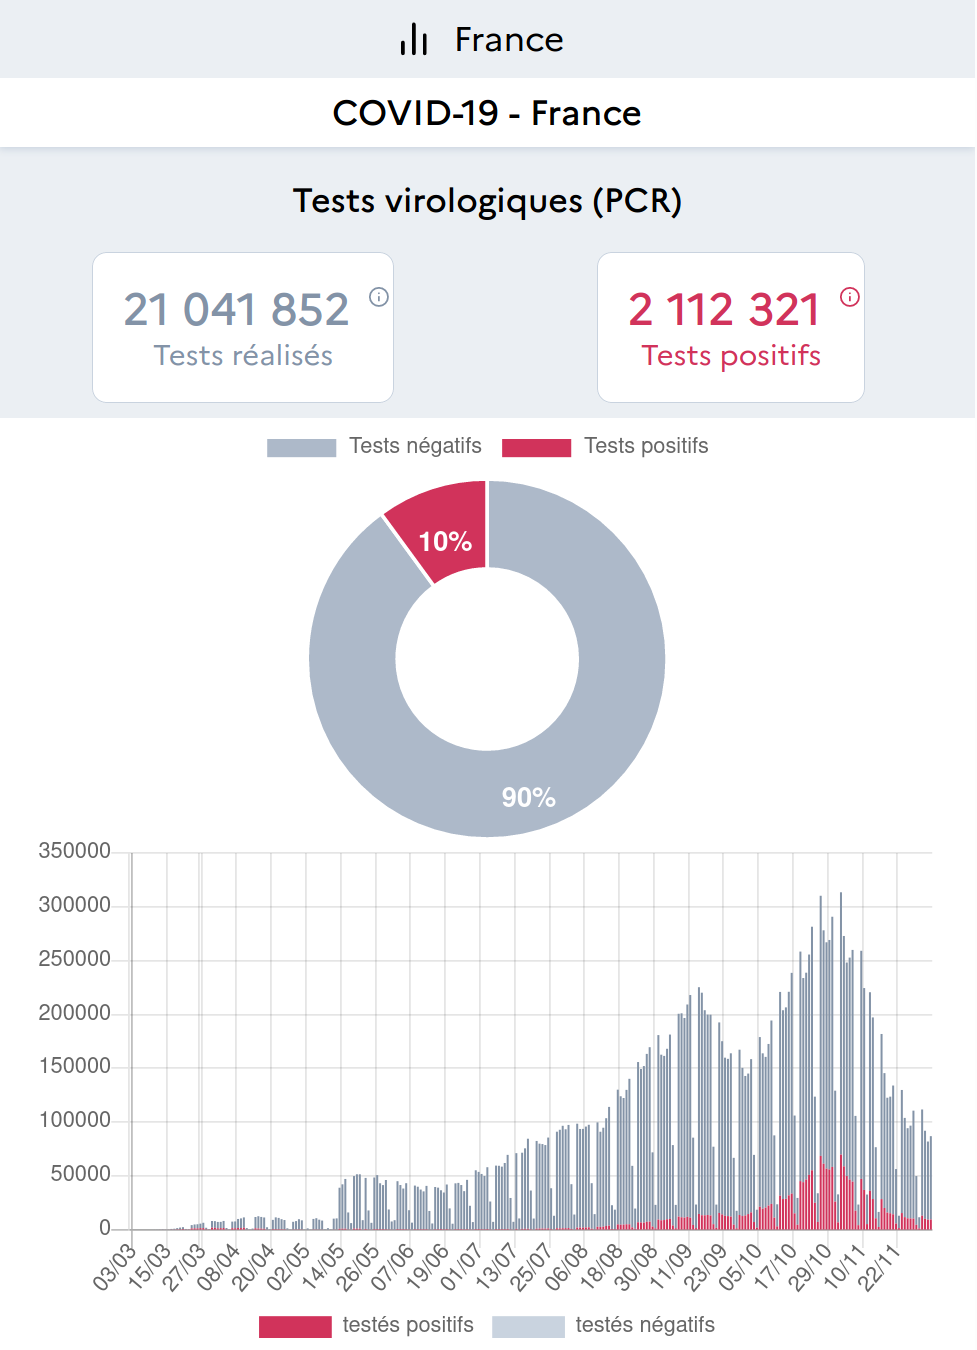
\includegraphics[width=0.5\linewidth]{img/tableau_bord}
  \caption{Tableau de bord des données Covid-19}
  \label{etagere}  \end{center}
 
\end{minipage}
\end{figure}

Liens vers les bases de données:
\begin{itemize}
 \item \href{https://www.data.gouv.fr/fr/datasets/indicateurs-de-suivi-de-lepidemie-de-covid-19/}{https://www.data.gouv.fr/fr/datasets/indicateurs-de-suivi-de-lepidemie-de-covid-19/}
 \item \href{https://www.data.gouv.fr/fr/datasets/donnees-relatives-aux-resultats-des-tests-virologiques-covid-19/}{https://www.data.gouv.fr/fr/datasets/donnees-relatives-aux-resultats-des-tests-virologiques-...}
\end{itemize}

Les données ont été téléchargées et formatées pour faciliter le travail. Elles sont présentes dans deux fichiers \verb?source1.csv? et \verb?source2.csv?. Ces fichiers sont présents dans le dossier de travail.

~\

On définit les éléments suivants:
\begin{itemize}
 \item le \textbf{taux d'incidence} correspond au nombre de tests virologiques positifs pour \num{100000} habitants sur une semaine. Il est calculé de la manière suivante : \\ \verb?taux_incidence=(100000*nb_cas_positif)/population?,
 \item le \textbf{taux de positivité} correspond au nombre de personnes testées positives sur une semaine. Il est calculé de la manière suivante : \\ \verb?taux_positivite=(100*nb_cas_positifs)/nb_tests?,
 \item la population française est d'environ \num{67000000} habitants.
\end{itemize}

\section*{Lecture et analyse de la première base de données}

\begin{enumerate}
\item  Mettre en en-tête du fichier les éléments suivants:
 \begin{itemize}
  \item \verb?import matplotlib.pyplot as plt?
  \item \verb?from datetime import datetime, timedelta?
 \end{itemize}
 
\item Proposer une fonction \verb?get_max(liste)? qui permet de déterminer le maximum, en valeur absolue, de la liste \verb?liste?. Tout le DS, sauf la dernière question, peut être traité même si vous ne répondez pas à cette question.

\begin{solution}~\ \\
\begin{minted}{python}
def get_max(liste):
    maximum=abs(liste[0])
    for valeur in liste:
        if abs(valeur)>maximum:
            maximum=abs(valeur)
    return maximum
\end{minted}
\end{solution}


% \begin{enumerate}
\item[3.1] Écrire un script python permettant de lire le contenu du fichier \verb?source1.csv?, et de stocker son contenu dans une liste dont chaque élément serait une ligne du contenu du fichier (il est recommandé d'utiliser les fonctions \verb?.read()? et \verb?.split()?). Afficher les deux premières lignes.

 \begin{solution}~\ \\
  \begin{minted}{python}
fichier=open('source1.csv','r')
contenu=fichier.read()
fichier.close()
	
lignes=contenu.split('\n')

print(lignes[0:2])
 \end{minted}
\end{solution}

L'exécution du script affiche le résultat suivant :
\begin{minted}{python}
['"extract_date","tx_incid","R","taux_occupation_sae","tx_pos"',
 '"2020-06-01",5.07875325643739,0.84,25.1,1.5664523487587']
\end{minted}

Dans cette liste, chaque ligne est comprise entre \verb?'? et \verb?'?. À l'intérieur de chaque ligne, les données de chacune des colonnes sont séparées par des \verb?,?. 

\item[3.2] Après avoir découpé la deuxième ligne selon ce séparateur, stocker son contenu dans une liste appelée \verb?data?. 

 \begin{solution}~\ \\
\begin{minted}{python}
data=lignes[1].split(",")
 \end{minted}
\end{solution}
% \end{enumerate}

\setcounter{enumi}{3}
\item Créer trois variables comme suit (attention de bien recopier les commandes) :
\begin{itemize}
 \item la date du test : \verb?jour_test = datetime.strptime(data[0], '"%Y-%m-%d"')?
 \item le taux d'incidence : \verb?taux_incidence=float(data[1])?
 \item le taux de positivité : \verb?taux_positivite=float(data[4])?
\end{itemize}

Afficher ces valeurs pour la première semaine.

 \begin{solution}~\ \\
\begin{minted}{python}
jour_test = datetime.strptime(data[0], '"%Y-%m-%d"')
taux_incidence=float(data[1])
taux_positivite=float(data[4])
print(jour_test,taux_incidence,taux_positivite)
 \end{minted}
\end{solution}

L'exécution du script affiche le résultat suivant:\\
\verb?2020-06-01 00:00:00 5.07875325643739 1.5664523487587?

\item Déterminer le nombre de tests, \verb?nb_tests?, effectués durant la première semaine à partir des données précédentes et grâce aux équations présentées en introduction. Nous ne garderons que la valeur entière de ce résultat.

 \begin{solution}~\ \\
$taux_{incidence}=\frac{100000*nb_{cas\ positif}}{population}$

$taux_{positivite}=\frac{100*nb_{cas\ positif}}{nb_{tests}}$,

$nb_{cas\ positif}=\frac{taux_{incidence}*population}{100000}$

$nb_{tests}=\frac{100*nb_{cas\ positifs}}{taux_{positivite}}$,

Donc,

$nb_{tests}=\frac{100*\frac{taux_{incidence}*population}{100000}}{taux_{positivite}}$.


\begin{minted}{python}
population=67000000
nb_tests=int((100*taux_incidence*population/100000)/taux_positivite)
print(nb_tests)
 \end{minted}
\end{solution}

L'exécution du script affiche le résultat suivant:\\
\verb?217227?

\item En utilisant les méthodes précédentes, créer deux listes \verb?liste_dates_tests1? et \verb?liste_nb_tests1? et y stocker les dates et le nombre de tests pour chaque semaine.

\begin{solution}~\ \\
\begin{minted}{python}
liste_dates_tests1=[]
liste_nb_tests1=[]
for ligne in lignes[1:-1]:
    data=ligne.split(",")
    jour_test = datetime.strptime(data[0], '"%Y-%m-%d"')
    liste_dates_tests1.append(jour_test)
    taux_incidence=float(data[1])
    taux_positivite=float(data[4])
    nb_tests=(100*taux_incidence*population/100000)/taux_positivite
    liste_nb_tests1.append(int(nb_tests))
\end{minted}
\end{solution}

\item Tracer la courbe du nombre de tests en fonction de la date. (Une date telle que nous l'avons codée plus haut peut être utilisée comme une abscisse classique.)

\begin{solution}~\ \\
\begin{minted}{python}
plt.plot(liste_dates_tests1,liste_nb_tests1)
\end{minted}
\end{solution}

\section*{Lecture et analyse de la deuxième base de données}

% \begin{enumerate}

\item[8.1] Lire le contenu du fichier \verb?source2.csv?, et stocker son contenu dans une liste dont chaque élément serait une ligne du contenu du fichier. Afficher les deux premières lignes.

\begin{solution}~\ \\
\begin{minted}{python}
fichier_test=open('source2.csv','r')
contenu=fichier_test.read()
fichier_test.close()

lignes=contenu.split('\n')

print(lignes[0:2])
\end{minted}
\end{solution}

L'exécution du script affiche le résultat suivant :
\begin{minted}{python}
['fra;week;P_f;P_h;P;T_f;T_h;T;cl_age90', 'FR;2020-S21;64;56;125;5263;6192;11683;09']
\end{minted}

Dans cette liste, chaque ligne est comprise entre \verb?'? et \verb?'?. À l'intérieur de chaque ligne, les données de chacune des colonnes sont, cette fois-ci, séparées par des \verb?;?. 

\item[8.2] Après avoir découpé la deuxième ligne selon ce séparateur, stocker son contenu dans une liste appelée \verb?data?. Afficher la dernière valeur de \verb?data?.
% \end{enumerate}

\begin{solution}~\ \\
\begin{minted}{python}
data=lignes[1].split(';')
print(data[-1])
\end{minted}
\end{solution}

La dernière colonne, ayant pour la première semaine la valeur \verb?09? indique la tranche d'âge de la personne testée (ici entre 0 et 9 ans). Il y a donc les catégories suivantes:
\begin{itemize}
 \item \verb?09?: âge entre 0 et 9 ans,
 \item ...
 \item \verb?89?: âge entre 80 et 89 ans,
 \item \verb?90?: âge de 90 ans et plus,
 \item \verb?0?: tous les âges.
\end{itemize}

Afin de comparer les résultats avec la base précédente, il faut prendre en compte toutes les tranches d'âge. C'est ce qui sera affiché lorsque cette colonne aura la valeur \verb?0?.

\setcounter{enumi}{8}
\item Créer trois variables comme suit (attention de bien recopier les commandes) et les stocker dans deux listes \verb?liste_dates_tests2? et \verb?liste_nb_tests2? (SEULEMENT SI la valeur \verb?data[8]=0?).

\begin{itemize}
 \item numéro de la semaine à laquelle a eu lieu le test : \verb?sem=data[1][-2:]?
 \item jour du test (on ajoute le nombre de semaines passées au 1er janvier 2020) :\\ \verb?jour_test = datetime(2020, 1, 1)+timedelta(weeks=int(sem))?
 \item le nombre de tests (il est stocké dans la colonne nommée \verb?T?) : \verb?nb_tests = int(data[7])?
\end{itemize}

\begin{solution}~\ \\
\begin{minted}{python}
liste_dates_tests2=[]
liste_nb_tests2=[]
for ligne in lignes[1:-1]:
    data=ligne.split(";")
    if data[8]=='0':
        sem=data[1][-2:]
        jour_test = datetime(2020, 1, 1)+timedelta(weeks=int(sem))
        liste_dates_tests2.append(jour_test)
        nb_tests=int(data[7])
        liste_nb_tests2.append(nb_tests)
\end{minted}
\end{solution}

\item Tracer la courbe du nombre de tests en fonction de la date. (Une date telle que nous l'avons codée plus haut peut être utilisée comme une abscisse classique.)

\begin{solution}~\ \\
\begin{minted}{python}
plt.plot(liste_dates_tests2,liste_nb_tests2)
plt.show()
\end{minted}
\end{solution}

Le 1er janvier 2020, n'étant pas un dimanche, nous obtenons un léger décalage entre les deux courbes.

\item En sachant que le dimanche précédent le 1er janvier 2020 était le 29 décembre 2019, modifier le code précédent pour prendre en compte ce décalage et tracer à nouveau la courbe. (La réponse à cette question n'est pas nécessaire pour traiter la suite.)

\begin{solution}~\ \\
\begin{minted}{python}
liste_dates_tests2=[]
liste_nb_tests2=[]
for ligne in lignes[1:-1]:
    data=ligne.split(";")
    if data[8]=='0':
        sem=data[1][-2:]
        jour_test = datetime(2019, 12, 29)+timedelta(weeks=int(sem))
        liste_dates_tests2.append(jour_test)
        nb_tests=int(data[7])
        liste_nb_tests2.append(nb_tests)

plt.plot(liste_dates_tests2,liste_nb_tests2)
plt.show()
\end{minted}
\end{solution}

\section*{Comparaison des deux courbes}

L'objectif de cette partie est de déterminer l'erreur relative entre les données calculées. Avant de comparer les deux bases, on constate que leur remplissage n'a pas démarré en même temps, la première date stockée n'étant pas la même.

\item Créer une liste \verb?liste_dates_ecarts?, contenant les dates des tests et une liste \verb?liste_ecarts? contenant la différence entre le nombre de tests déterminé à partir de \verb?liste_nb_tests1? et celui déterminé à partir de \verb?liste_nb_tests2?. Il ne faudra remplir la liste que si les deux valeurs du nombre de tests sont disponibles à cette date.

\begin{solution}~\ \\
\begin{minted}{python}
liste_dates_ecarts=[]
liste_ecarts=[]
for i,date in enumerate(liste_dates_tests2):
     if date in liste_dates_tests1:
         liste_dates_ecarts.append(date)
         liste_ecarts.append(liste_nb_tests2[i]-liste_nb_tests1[liste_dates_tests1.index(date)])\end{minted}
\end{solution}

\item Tracer cet écart en fonction de la date (il faudra commenter, dans le script, l'affichage des courbes précédentes afin de ne pas écraser celle-ci.)

\begin{solution}~\ \\
\begin{minted}{python}
plt.figure(2)
plt.plot(liste_dates_ecarts,liste_ecarts)
plt.show()
\end{minted}
\end{solution}

\item Déterminer, à l'aide de la fonction déterminée à la première question, le maximum, en valeur absolue, de \verb?liste_ecarts? et de \verb?liste_nb_tests1? et en déduire l'erreur relative maximale en \% entre \verb?liste_nb_tests1? et \verb?liste_nb_tests2?. Vous afficherez:
\begin{itemize}
 \item le maximum de \verb?liste_ecarts?,
 \item le maximum de \verb?liste_nb_tests1?,
 \item l'erreur en \%.
\end{itemize}


\begin{solution}~\ \\
\begin{minted}{python}
print('Nb écarts',get_max(ecarts))
print('Nb tests',get_max(nb_tests1))

print('Erreur relative pourcent',100*get_max(ecarts)/get_max(nb_tests1))
\end{minted}
\end{solution}

\end{enumerate}
\end{document}
